
\section{Teoria de Jogos, Coordenação e Planejamento}
\begin{frame}

\begin{center}
{\huge Capítulo 4 -- Teoria de Jogos e  Coordenação}

3 partes fundamentais:

\begin{enumerate}
  \item Teoria de Jogos
  \item Coordenação
  \item Planejamento
\end{enumerate}
Nesta ordem
\end{center}

\end{frame}

%-----------------------------------------------------------


%-----------------------------------------------------------


\section{Estratégias de Jogos}
\begin{frame}

    \frametitle{Teoria de Jogos}
    \begin{itemize}
    \pause
      \item SMA como um comunidade que coopera, disputa e \textit{compete} 
      \pause
      \item Asssim uma métrica entre todos os agentes (\textit{local})
       é necessária para
      se levantar um valor \textit{global} de eficiência
    
    \end{itemize}
\end{frame}


%-----------------------------------------------------------

\subsection{Teoria de Jogos Aplicado a SMA}
\begin{frame}

    \frametitle{Dilema do Prisioneiro}
   
    
\begin{quotation}
        Houve um assassinato e existem dois suspeitos, A e B. Se não se conseguir provar quem foi o assassino, a pena seria de apenas 6 meses por porte de arma.
Se um suspeito acusa (trair ou delatar) o outro e este não se defender (fica calado), então  será condenado a 10 anos. Assim, o traidor que colabora com a polícia sairá livre. Se os dois se acusarem mutuamente a pena é de 5 anos para cada um, pois a
polícia não acredita em nenhum dos dois.
    \end{quotation}
    
    
    
\begin{itemize}
  
  \item Como os suspeitos não conhecem a \textit{Teoria dos Jogos}, o normal será que se acusem mutuamente
    
  \item Os suspeitos serão interrogados em separado e não tem acesso a(s) resposta(s) do outro

\item Sim, plural: \textit{rodadas} ou \textit{jogadas} de respostas!
\end{itemize}

   
\end{frame}

%-----------------------------------------------------------

\begin{frame}

    \frametitle{Coletando os Dados: Dilema do Prisioneiro}
    
    
      \begin{center}
        \begin{tabular}{p{2cm} || p{3cm} | p{3cm}} \hline \hline
  & Prisioneiro B nega   &  Prisioneiro B delata   \\ \hline \hline
        Prisioneiro A nega (silêncio ou não-confessa)  &  Ambos condenados a 6 meses  & A é condenado a 10 anos e B é livre   \\ \hline 
         Prisioneiro A delata (acusa ou trai)     & B é condenado a 10 anos e A é livre & Ambos são condenados a 5 anos \\ 
         \hline \hline
        \end{tabular}
      \end{center}

\end{frame}
%-----------------------------------------------------------


\begin{frame}

    \frametitle{Hipóteses: Dilema do Prisioneiro}
    
    
    \begin{itemize}
      \item  Vamos supor que ambos os prisioneiros são completamente egoístas e a sua única meta é reduzir a sua própria estadia na prisão. Como prisioneiros têm duas opções:
      
      \begin{enumerate}
         \item cooperar com o seu cúmplice e permanecerem calados
         \item ou trair o seu cúmplice e confessar que foi o outro
       \end{enumerate}   
       
       \begin{itemize}
         \item   O resultado de cada escolha depende da escolha do cúmplice.     
         \item   Infelizmente, um não sabe o que o outro escolheu fazer. 
       \end{itemize}
       
       \item Inclusive se pudessem falar entre si, não poderiam estar seguros de confiar um no outro (um diria ao outro que era melhor ficarem calados, e depois trairiam o outro)        
       
    \end{itemize}


\end{frame}

%-----------------------------------------------------------

\begin{frame}
    \frametitle{Analisando os fatos:}

%\begin{small}
\begin{quotation}
Se se esperar que o cúmplice escolha cooperar com ele e permanecer em silêncio, a opção óptima para o primeiro seria confessar, o que significaria que seria libertado imediatamente, enquanto o cúmplice terá que cumprir uma pena de 10 anos. Se espera que seu cúmplice decida confessar, a melhor opção é confessar também, já que ao menos não receberá a pena completa de 10 anos, e apenas terá que esperar 5, tal como o cúmplice. Se ambos decidirem cooperar e permanecerem em silêncio, ambos serão libertados em apenas 6 meses.
\end{quotation}
%\end{small}


\end{frame}

%-----------------------------------------------------------

\begin{frame}
    \frametitle{Análise: Dilema do Prisioneiro}

   \begin{itemize}
     \item Confessar é uma \textit{estratégia dominante} para ambos os jogadores. Seja qual for a escolha do outro jogador, podem reduzir sempre sua sentença confessando. 
   
  \item Por infelicidade para os prisioneiros, isto conduz a um resultado ruim, no qual ambos acusam seus companheiros e ambos recebem longas condenações. \textcolor{red}{Aqui se encontra o ponto-chave do dilema.} 
  
  \item O resultado das acusações individuais produz um resultado que não é óptimo no sentido de Pareto; existe uma situação tal que a utilidade de um dos detidos poderia melhorar (ou mesmo a de ambos) sem que isto implique uma piora para o resto. 
  
  \item Ou seja, o resultado no qual ambos os detidos não confessam (silêncio) dominam o resultado no qual os dois escolhem confessar.

   \end{itemize}
   
\end{frame}


%-----------------------------------------------------------


\begin{frame}
    \frametitle{Análise: Dilema do Prisioneiro}

 \begin{itemize}
  
 
   \item Perspectiva de interesse ótimo para o grupo (i.é. dois prisioneiros), o resultado correto é que  ambos cooperassem (entre si, ficando calados).
   Pois,  isto reduziria o tempo total de pena do grupo a um total de um ano (6 meses para cada um).

   \item  Qualquer outra decisão seria pior para ambos se se considerar conjuntamente.

\item Se um jogador tiver uma oportunidade para castigar o outro jogador ao confessar (delatar o outro), então um resultado cooperativo (um vai para prisão apenas?) pode manter-se.

\pause
   
   
\item Este jogo possui como solução do ponto de vista \textit{Ótimo de Pareto} a estratégia:
A e B negam (ficam calados!)

\pause
   
   
\item Este jogo possui como 
\textit{Equilíbrios de Nash} a estratégia: 
A e B delatam: neste caso, é o \textit{equilíbrio dominante}.

\item Porquê é chamado de \textit{Equilíbrios de Nash}?
     
 \end{itemize}
 
 %%Apesar disso, se continuarem no seu próprio interesse egoísta, cada um dos dos prisioneiros receberá uma dura pena.
 
% A forma iterada de este jogo (mencionada mais abaixo) oferece uma oportunidade para este tipo de castigo. Nesse jogo, se o cúmplice trai e confessa uma vez, pode-se castigá-lo traindo-o na próxima. Assim, o jogo iterado oferece uma opção de castigo que está ausente no modo clássico do jogo.


\end{frame}
%-----------------------------------------------------------


\begin{frame}
    \frametitle{Formulação: Dilema do Prisioneiro}

\begin{itemize}
  \item $Jogadores = \{A,B\}$
  \item Espaço de estratégia do jogo: $S_A = \{confessa, \:\: nega\}$ e  $S_B = \{confessa, \:\: nega\}$
  \item Espaço do jogo: $S = \{ (nega, nega), (nega,confessa), (confessa, nega), (confessa, confessa) \}$
  \item Função de utilidade: $u_i: S \rightarrow R$ onde $i \in \{A,B\}$
  
  \item No caso $u_A (s): S \rightarrow R$ e $u_B (s): S \rightarrow R$

  \item Assim o mapeamento desta função de utilidade dos jogadores $A$ e $B$:
  
  \begin{itemize}
    \item Para o jogador A:  $u_A (nega, nega) = -1$, $u_A(nega, confessa) = 0$, $u_A(confessa, nega) = -10$  e  $u_A(confessa, confessa) = -5$
  
    \item  Para o jogador B:  $u_B(nega, nega) = -1$, $u_B(nega, confessa) = -10$, $u_B(confessa, nega) = 0$  e  $u_B(confessa, confessa) = -5$
    
  \end{itemize}
  
\end{itemize}


\end{frame}


%-----------------------------------------------------------
\begin{frame}
\frametitle{Construindo uma Matriz de Ganhos:}


  \begin{center}
    \begin{tabular}{c||c|c}
    \hline \hline
               & B Nega & B Delata  \\     \hline \hline
     A Nega\footnote{Ficar calado.}    &   (-1,-1)     &  (-10, 0)  \\     \hline 
     A Delata\footnote{Trair o outro.}  &    (0, -10)   &  (-5,-5)   \\
         \hline \hline
    \end{tabular}
  \end{center}

\begin{itemize}
  \item Sendo \textit{egoísta}, a melhor estratégia é delatar seu companheiro e este não se defender
  
  \item Assim, seja qual for a opção do adversário, individualmente, qualquer um se sai melhor traindo ou delatando o outro
  
  \item Ambos chegam individualmente a conclusão \textbf{racional}: \textit{trair}!
  
  \item Nesta lógica individual, as penas somam 10 anos de prisão!
    
  \end{itemize}


\end{frame}

%----------------------------------------------------------

\begin{frame}
\frametitle{Reflexões: Dilema do Prisioneiro}

\begin{itemize}
  \item E se os jogadores aprendessem a \textit{cooperar} após sucessivas jogadas?

  \item Assim suge o \textit{princípio da reciprocidade}, onde o jogador $B$ 
  deve cooperar com $A$ seguindo-o na sua escolha

\pause 
  \item Do livro \textit{A evolução da cooperação: o dilema do prisioneiro e a teoria de jogos} (1984),  de Robert Axelrod, tem-se a terminologia do \textit{ganha-ganha}: 
    
  \begin{center}
    \begin{tabular}{c||p{3cm}|p{3cm}}
    \hline \hline
                & B Coopera & B Delata  \\     \hline \hline
     A Coopera  &   ganha -- ganha     & perda substancial -- ganho substancial  \\     \hline 
     A Delata   &    	ganho substancial -- perda substancial &  	perde -- perde   \\
         \hline \hline

    \end{tabular}
  \end{center}

\end{itemize}

\end{frame}
%----------------------------------------------------------

\begin{frame}
\frametitle{Reflexões: Dilema do Prisioneiro}

\begin{itemize}
\item Outros exemplos: corrida de bicicleta (\textit{Tour de France}, Giro na Itália, etc)  onde há um revezamento na liderança para se poupar, nem se assume a liderança isolada para não se desgastar!

\item O problema da troca de malas

\item \textit{The refund}: recompensa em dizer a verdade 

\item ... ver outros exemplos e TODOS se identificam

\item Como integrar isto a SMAs?
\end{itemize}

\end{frame}


%----------------------------------------------------------
%----------------------------------------------------------

%%% longe
\section{Coordenação}


\begin{frame}
\frametitle{Coordenação}



\end{frame}


%-----------------------------------------------------------


\subsection{Jogos de Coordenação}

\begin{frame}
\frametitle{Jogos de Coordenação}

pag 23


\end{frame}


%-----------------------------------------------------------
\subsection{Convenção Social}

\begin{frame}
\frametitle{Convenção Social}

pag 24


\end{frame}
%-----------------------------------------------------------

\subsection{Papel Social}

\begin{frame}
\frametitle{Papel Social}

pag 25


\end{frame}



%-----------------------------------------------------------
\subsection{Grafos de Coordenação}

\begin{frame}
\frametitle{Grafos de Coordenação}

pag 26


\end{frame}
%-----------------------------------------------------------


\subsubsection{Coordenação por Eliminação de Variáveis}

\begin{frame}
\frametitle{Coordenação por Eliminação de Variáveis}

pag 28


\end{frame}
%-----------------------------------------------------------


\subsubsection{Coordenação por Troca de Mensagens}

\begin{frame}
\frametitle{Coordenação por Troca de Mensagens}

pag 28


\end{frame}
%-----------------------------------------------------------

\section{Planejamento}


\begin{frame}
\frametitle{Fundamentos de Planejamento}



\end{frame}
%-----------------------------------------------------------


\subsection{Abordagens ao Planejamento Multiagente -- SMAs}

\begin{frame}
\frametitle{Abordagens ao Planejamento de SMAs}

\begin{block}{}
 
\begin{itemize}
  \item Coordenação central: controla todos os subplanos
  \item Esquemas de controle distribuído\\
        Conhecimento parcial dos planos de outros agentes
  \item Planejamento Global Negociado

\begin{itemize}
  \item Compartilhamento de todos os planos
  \item Ajuste local para a realização de objetivos comuns

\end{itemize}

\item Modelagem Explícita da Equipe de Agentes
\begin{itemize}
  \item Compromissos conjuntos
   \item Crenças, desejos e intenções comuns

\end{itemize}
\end{itemize}
\end{block}

\end{frame}

%-----------------------------------------------------


\subsection{Exemplos de Coordenação SMAs}

\begin{frame}
\frametitle{Exemplo de Coordenação SMAs}

\begin{figure}[!ht]
\centering
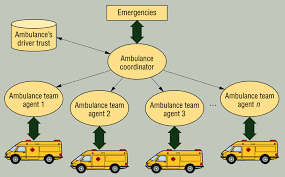
\includegraphics[height =.6\textheight,width=.7\textwidth]{figuras/coordenacao_agentes01.png}
\caption{Coordenação de agentes $\equiv $   SMA}
%\label{ag_01}
\end{figure}
 \end{frame}

%-----------------------------------------------------------

\begin{frame}
\frametitle{Exemplo de Coordenação SMAs}

\begin{figure}[!ht]
\centering
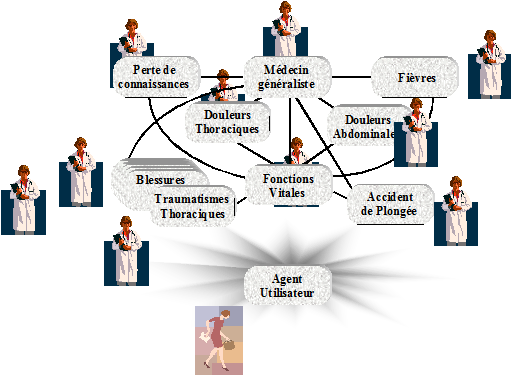
\includegraphics[height =.6\textheight,width=.7\textwidth]{figuras/coordenacao_agentes02.png}
\caption{Coordenação de agentes $\equiv $   SMA}
%\label{ag_01}
\end{figure}
 
\end{frame}


%-----------------------------------------------------------
